\section{ReactJS}
\label{sec:reactJS}
ReactJS é uma biblioteca NodeJS de código aberto criada pelo Facebook em 2011 para o desenvolvimento de interfaces \textit{web} em JavaScript e/ou Typescript. Comparando-o com outras bibliotecas e \textit{frameworks} para o desenvolvimento \textit{web front-end}, constata-se que seu diferencial se encontra na abordagem de construção da interface baseada em componentes atualizados e sincronizados de forma muito mais otimizada.

A arquitetura base de um projeto ReactJS consiste em uma estrutura hierárquica de componentes onde cada componente representa uma parte da interface final do usuário, que possui sua própria lógica e aparência isolada de outros componentes. Nesse contexto, um dos caminhos ideais da construção do código encontra-se no princípio de “separação de conceitos”, onde cada seção(ou componente) é responsável por lidar com apenas um assunto separadamente e nada além disso, resultando em uma arquitetura mais modular e escalável \cite{Qawwas2022}.

Empiricamente, cada componente React é uma função que retorna uma pequena porção de código HTML, que é estilizado por código CSS e passível de ser modificado pelas lógicas em JavaScript/TypeScript que existem dentro dessa mesma função, permitindo assim que esse pedaço de interface usufrua de todas funcionalidades que essas linguagens de programação oferecem.

\begin{figure}[H]
    \centering
    \caption{Código exemplo em ReactJS.}
    \label{fig:reactJS}
    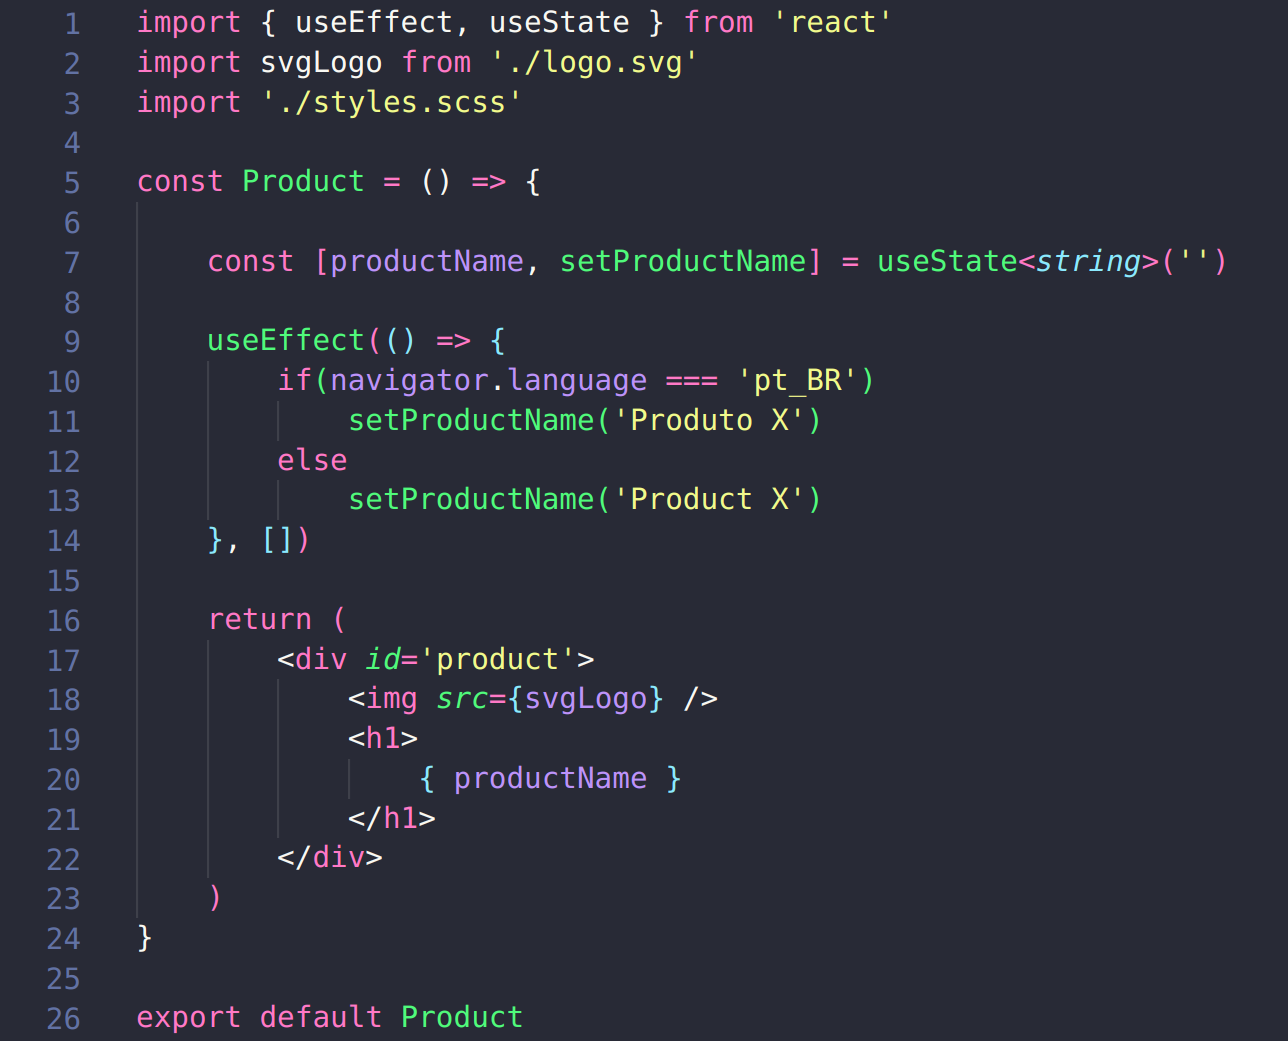
\includegraphics[width=.7\textwidth]{data/figures/react.png}
    \fonte{Autor}
\end{figure}

Atualmente, de acordo com a pesquisa Developer Survey realizada pela \citeonline{Exchange2023}, ReactJS é a biblioteca de desenvolvimento \textit{web} mais utilizada no âmbito profissional, refletindo o amplo apoio que a biblioteca possui em novas funcionalidades e resolução de problemas.